\begin{tikzpicture}[scale=0.9]

%Couleurs
\def \colelastomere{yellow!60}
\def \colreservoir{black!50}

%Dimentions du réservoir et de la jupette
\def \epaisseurreservoir{.125}
\def \ldroit{3}
\def \laxe{1.}
\def \tjupette{0.125}
\def \ljupette{4}
\def \rayonint{0.6*\ljupette}

%Définition de l'espace entre les éléments de la soudure
\def \espace{0.125}
\def \lsoudure{0.75}
\def \telastomere{0.2}

\tikzstyle{loosely dashed}=      [dash pattern=on 18pt off 5pt on 5pt off 5 pt]

%paroi du réservoir
\draw[black,fill=\colreservoir] (0,\rayonint) arc (90:180:\rayonint) -- ++ (- \epaisseurreservoir,0) arc (180:90:\rayonint+\epaisseurreservoir) -- ++ (\ldroit,0) -- ++ (0,-\epaisseurreservoir) -- cycle; 
\draw[black,decorate,decoration=random steps] (\ldroit,\rayonint) -- ++ (0,-\rayonint);

%Axe
\draw[black,thick,loosely dashed] (-\rayonint-\laxe,0) -- ++ (\rayonint+\ldroit+2*\laxe,0);

%Éléments chauffants
\draw[black,very thick] (0,\rayonint+\epaisseurreservoir+\espace) -- ++(\lsoudure,0);
\draw[black,very thick] (0,\rayonint+\epaisseurreservoir+3*\espace+\telastomere) -- ++(\lsoudure,0);

%Élastomère
\draw[black,fill=\colelastomere] (0,\rayonint+\epaisseurreservoir+2*\espace) -- ++(\lsoudure,0) -- ++(0,\telastomere) -- ++ (-\lsoudure,0) -- cycle;

%Jupette
\draw[black,fill=\colreservoir] (\lsoudure,\epaisseurreservoir+4*\espace+\telastomere+\rayonint)  -- ++ (-\ljupette,0) -- ++ (0,\tjupette) -- ++(+\ljupette,0)  -- cycle; 

%Identification
\draw[black,thin] (\lsoudure,\epaisseurreservoir+4*\espace+\telastomere+\rayonint+0.5*\tjupette) -- ++ (1,2*\espace) node[right] {Jupette};

\draw[black,thin] (\lsoudure,\epaisseurreservoir+3*\espace+\telastomere+\rayonint) -- ++ (1,-\espace-0.5*\telastomere) ;

\draw[black,thin] (0,\epaisseurreservoir+2*\espace+0.5*\telastomere+\rayonint) -- ++ (-1,-0.5*\telastomere) node[left] {Élastomère};

\draw[black,thin] (\lsoudure,\epaisseurreservoir+\espace+\rayonint) -- ++ (1,\espace+0.5*\telastomere) node[right] {Adhésif};

\draw[black,thin] (0.25*\ldroit,\rayonint) -- ++ (-0.5*\lsoudure,-0.375*\rayonint) node[below] {Réservoir};

\node[inner sep=0pt] (SaturnV) at (9,2)
{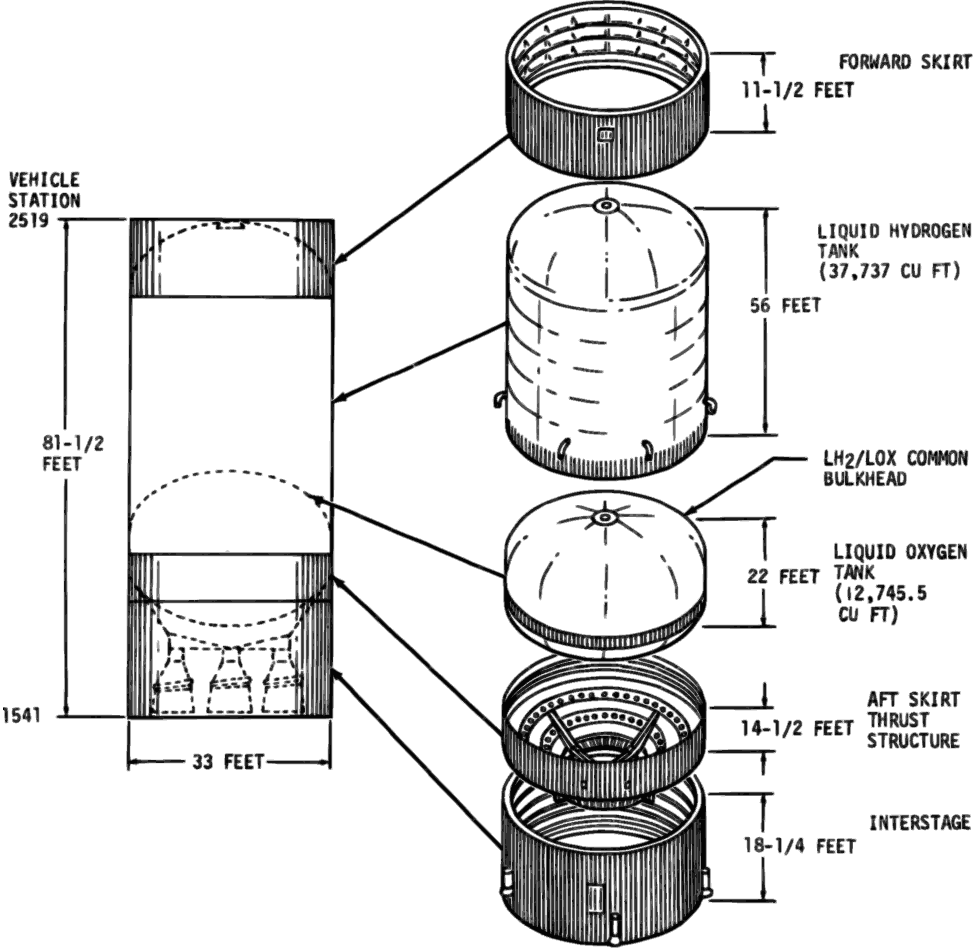
\includegraphics[width=.5\textwidth]{SaturnV_stage2.pdf}};

\node (a) at (1,-3) {a)};
\node (b) at (9,-3) {b)};

\draw[red,very thick] (6.6,1) ellipse [x radius=1.5,y radius=0.4];
\draw[red,very thick] (6.6,3.9) ellipse [x radius=1.5,y radius=0.4];

\end{tikzpicture}